\chapter{Miara}
\label{chap:miara}

\section{Funkcje zbioru i addytywność}
\label{sec:funkcje-zbioru-addytywnosc}

\begin{definicja}[Funkcja zbioru]
Niech $\mathcal{A}\subseteq\mathcal{P}(X)$ będzie rodziną zbiorów.
Odwzorowanie
\[
  \mu:\mathcal{A}\longrightarrow[0,+\infty]
\]
nazywamy funkcją zbioru.
\end{definicja}

\begin{definicja}[Skończona addytywność]
Funkcja zbioru $\mu:\mathcal{A}\to[0,+\infty]$ jest skończenie
addytywna, jeżeli dla $A,B\in\mathcal{A}$ takich, że
$A\cap B=\varnothing$ i $A\cup B\in\mathcal{A}$, zachodzi
\begin{equation}
  \mu(A\cup B)=\mu(A)+\mu(B).
  \label{eq:skonczona-addytywnosc}
\end{equation}
\end{definicja}

\begin{definicja}[Przeliczalna addytywność]
\label{def:przeliczalna-addytywnosc}
Funkcja zbioru $\mu:\mathcal{A}\to[0,+\infty]$ jest przeliczalnie
addytywna, jeżeli dla każdego ciągu parami rozłącznych zbiorów
$A_n\in\mathcal{A}$, którego suma należy do $\mathcal{A}$, mamy
\begin{equation}
  \mu\left(\bigcup_{n=1}^{\infty}A_n\right)
  =\sum_{n=1}^{\infty}\mu(A_n).
  \label{eq:przeliczalna-addytywnosc}
\end{equation}
Parami rozłączne oznacza, że $A_n\cap A_m=\varnothing$ dla $n\neq m$.
\end{definicja}

\section{Miara i przestrzeń z miarą}
\label{sec:miara-przestrzen}

\begin{definicja}[Miara]
\label{def:miara}
Niech $(X,\mathcal{F})$ będzie przestrzenią mierzalną.
Miarą na sigma-ciele $\mathcal{F}$ nazywamy przeliczalnie addytywną
funkcję zbioru
\[
  \mu:\mathcal{F}\longrightarrow[0,+\infty]
\]
spełniającą warunek $\mu(\varnothing)=0$.
\end{definicja}

\begin{definicja}[Przestrzeń z miarą]
Trójkę $(X,\mathcal{F},\mu)$, gdzie $\mathcal{F}$ jest sigma-ciałem
podzbiorów $X$, a $\mu$ jest miarą na $\mathcal{F}$,
nazywamy przestrzenią z miarą lub przestrzenią miarową.
Zbiory należące do $\mathcal{F}$ nazywamy zbiorami mierzalnymi.
\end{definicja}

\section{Własności miary}
\label{sec:wlasnosci-miary}

W tej części $(X,\mathcal{F},\mu)$ jest przestrzenią z miarą,
a wszystkie rozważane zbiory należą do $\mathcal{F}$.

\begin{fakt}[Skończona addytywność miary]
\label{fakt:miara-skonczona-addytywnosc}
Miara jest skończenie addytywna: jeżeli $A\cap B=\varnothing$, to
\[
  \mu(A\cup B)=\mu(A)+\mu(B).
\]
\end{fakt}

\begin{proof}
Połóżmy $A_1=A$, $A_2=B$ oraz $A_n=\varnothing$ dla $n\geq3$.
Zbiory tego ciągu są parami rozłączne. Z przeliczalnej addytywności
i warunku $\mu(\varnothing)=0$ otrzymujemy
\[
  \mu(A\cup B)
  =\mu\left(\bigcup_{n=1}^{\infty}A_n\right)
  =\sum_{n=1}^{\infty}\mu(A_n)=\mu(A)+\mu(B).
\]
\end{proof}

\begin{uwaga}
Indukcyjnie dla dowolnych parami rozłącznych zbiorów
$A_1,\ldots,A_n\in\mathcal{F}$ mamy
\[
  \mu\left(\bigcup_{k=1}^{n}A_k\right)=\sum_{k=1}^{n}\mu(A_k).
\]
\end{uwaga}

\begin{fakt}[Subtraktywność]
\label{fakt:miara-subtraktywnosc}
Jeżeli $A\subseteq B$ i $\mu(A)<+\infty$, to
\begin{equation}
  \mu(B\setminus A)=\mu(B)-\mu(A).
  \label{eq:miara-subtraktywnosc}
\end{equation}
\end{fakt}

\begin{proof}
Zbiory $A$ i $B\setminus A$ są mierzalne i rozłączne, a ich suma
jest równa $B$. Z faktu~\ref{fakt:miara-skonczona-addytywnosc} wynika
\begin{equation}
  \mu(B)=\mu(A)+\mu(B\setminus A).
  \label{eq:miara-rozklad-roznicy}
\end{equation}
Ponieważ $\mu(A)$ jest skończona, możemy ją odjąć i otrzymujemy
\eqref{eq:miara-subtraktywnosc}.
\end{proof}

\begin{fakt}[Miara sumy i przekroju]
\label{fakt:miara-suma-przekroj}
Dla dowolnych $A,B\in\mathcal{F}$ zachodzi
\begin{equation}
  \mu(A)+\mu(B)=\mu(A\cup B)+\mu(A\cap B).
  \label{eq:miara-suma-przekroj}
\end{equation}
\end{fakt}

\begin{proof}
Z rozkładu $A=(A\cap B)\cup(A\setminus B)$ na zbiory rozłączne
otrzymujemy
\begin{align*}
  \mu(A)+\mu(B)
    &=\mu(A\cap B)+\mu(A\setminus B)+\mu(B)\\
    &=\mu(A\cap B)+\mu\bigl((A\setminus B)\cup B\bigr)\\
    &=\mu(A\cap B)+\mu(A\cup B).
\end{align*}
W drugim przejściu użyliśmy rozłączności $A\setminus B$ i $B$.
\end{proof}

\begin{fakt}[Monotoniczność]
\label{fakt:miara-monotonicznosc}
Jeżeli $A\subseteq B$, to $\mu(A)\leq\mu(B)$.
\end{fakt}

\begin{proof}
Z równości~\eqref{eq:miara-rozklad-roznicy} i nieujemności miary wynika
\[
  \mu(B)=\mu(A)+\mu(B\setminus A)\geq\mu(A).
\]
Sam rozkład~\eqref{eq:miara-rozklad-roznicy} nie wymaga założenia
o skończoności $\mu(A)$.
\end{proof}

\begin{fakt}[Przeliczalna podaddytywność]
\label{fakt:miara-podaddytywnosc}
Dla dowolnego ciągu zbiorów $A_n\in\mathcal{F}$ zachodzi
\begin{equation}
  \mu\left(\bigcup_{n=1}^{\infty}A_n\right)
  \leq\sum_{n=1}^{\infty}\mu(A_n).
  \label{eq:miara-podaddytywnosc}
\end{equation}
\end{fakt}

\begin{proof}
Połóżmy $B_1=A_1$ oraz dla $n\geq1$
\begin{equation}
  B_{n+1}=A_{n+1}\setminus\bigcup_{k=1}^{n}A_k.
  \label{eq:rozlacznienie-ciagu}
\end{equation}
Zbiory $B_n$ są mierzalne, parami rozłączne i spełniają $B_n\subseteq A_n$.
Ponadto
\[
  \bigcup_{n=1}^{\infty}B_n=\bigcup_{n=1}^{\infty}A_n:
\]
każdy punkt sumy należy do pierwszego zbioru $A_n$, w którym się pojawia,
a więc należy do odpowiedniego $B_n$.
Z przeliczalnej addytywności i monotoniczności miary otrzymujemy
\[
  \mu\left(\bigcup_{n=1}^{\infty}A_n\right)
  =\mu\left(\bigcup_{n=1}^{\infty}B_n\right)
  =\sum_{n=1}^{\infty}\mu(B_n)
  \leq\sum_{n=1}^{\infty}\mu(A_n).
\]
\end{proof}

\begin{figure}[htbp]
  \centering
  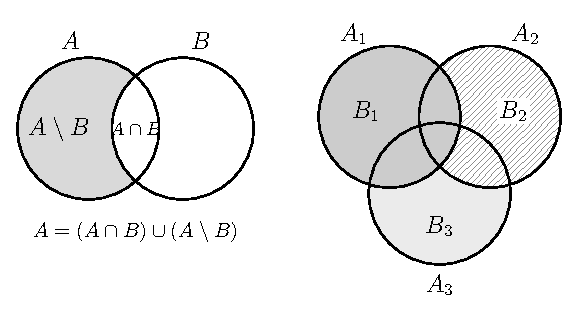
\includegraphics[width=0.93\textwidth]{roznica-i-rozlacznienie.pdf}
  \caption{Rozkład zbioru $A$ oraz rozłącznienie pierwszych trzech zbiorów ciągu.}
  \label{fig:roznica-i-rozlacznienie}
\end{figure}
